\documentclass{article}
\usepackage{tikz}
\begin{document}
	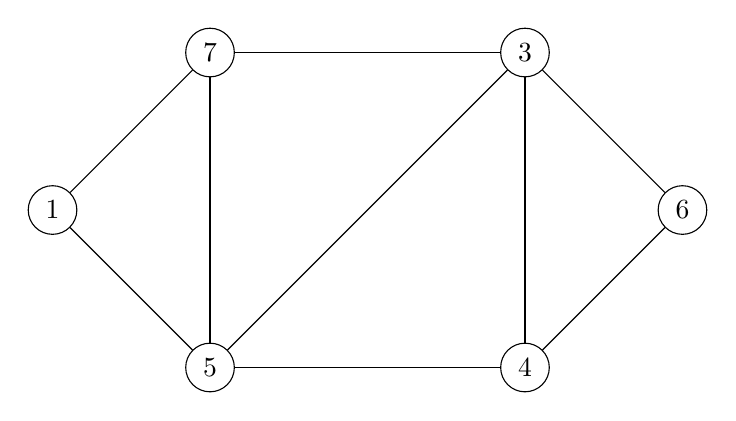
\begin{tikzpicture}
	\tikzstyle{node_style} = [circle,draw=black]
	\tikzstyle{edge_style} = [draw=black]
	\node[node_style] (v1) at (-2,2) {7};
	\node[node_style] (v2) at (2,2) {3};
	\node[node_style] (v3) at (4,0) {6};
	\node[node_style] (v4) at (2,-2) {4};
	\node[node_style] (v5) at (-2,-2) {5};
	\node[node_style] (v6) at (-4,0) {1};
	\draw[edge_style]  (v1) edge (v2);
	\draw[edge_style]  (v2) edge (v3);
	\draw[edge_style]  (v3) edge (v4);
	\draw[edge_style]  (v4) edge (v5);
	\draw[edge_style]  (v5) edge (v6);
	\draw[edge_style]  (v6) edge (v1);
	\draw[edge_style]  (v5) edge (v1);
	\draw[edge_style]  (v5) edge (v2);
	\draw[edge_style]  (v4) edge (v2);
	\end{tikzpicture}
\end{document}